\documentclass{article}
\usepackage{import}
\subimport{../}{preamble}
\begin{document}

\subsection{Decontamination of Tip Surfaces and Post-Fabrication Processing}

% Post-processing
After each batch of fabrications, tips are imaged using SEM to study surface morphology. Characterisation is necessary to determine the specific apex morphology but leads to contamination issues. Exposure to the electron beam is known to deposit layers of carbon onto samples. Despite washing tips in DI water and ethanol after deposition to remove any leftover chemical films, the surface of the tip inevitably contains carbon contamination after imaging. To ensure good electrical contact, AuNP tips must be cleaned before use. Although plasma cleaning is used to remove organics from the surface before fabrication surface oxidation can be detrimental to establishing electrical contact. Submerging tips in piranha solution (3\,H\subs2SO\subs4\,:\,1\,H\subs2O\subs2) for \SI{10}{\minute} proves to be an effective method for removing organics from the surface of the Au without introducing any adverse surface layers.%
\footnote{Piranha solution is a strong oxidising agent and works via H\subs2SO\subs4 quickly dehydrating organics. H\subs2SO\subs4 and H\subs2O\subs2 react to create oxygen radicals which oxidise the remaining carbon molecules into elemental carbon. The overall result is the decomposition of organic matter into carbon, CO\subs2 and water.}
Though it can still oxidise or hydroxylate surfaces this is to a lesser extent compared to plasma treatment. Tips treated with piranha solution electrically contacted more often than tips left untreated after SEM imaging.

\begin{figure}[bt]
\centering
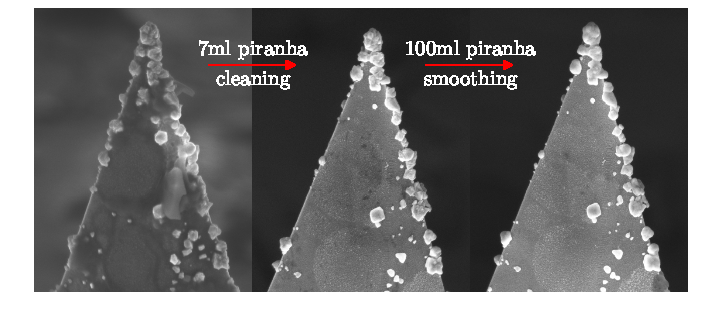
\includegraphics[clip=true, trim=20 20 0 0]{figures/tip_post_processing}
\caption[Post-processing effects of piranha solution.]{\textbf{Post-processing effects of piranha solution.} Low volume and temperature piranha solution removes organics from the Au surface while large volumes at \SI{120}{\celsius} also smooth the surface.}
\label{fig:tip_post_processing}
%\vspace{-5pt}
\end{figure}

% Temperature effects
The activity of piranha solution degrades over time with some indication that small volumes of the solution loses effectiveness after only \SI{15}{\minute}. During its initial stages, the piranha reaction is extremely exothermic with temperatures reaching up to \SI{120}{\celsius}. The overall temperature of the solution is determined by the volume of solution used. The heat generated in larger volumes takes longer to dissipate, maintaining a higher average solution temperature. The morphology of tips can be somewhat adjusted by exposing tips to piranha solution with varying temperatures and exposure times. Tips cleaned in small (\SI{5}{ml}) volumes show no changes in morphology whereas those treated in a large (\SI{100}{ml}) volumes are found to have smoothed surfaces, as seen in \figurename~\ref{fig:tip_post_processing}. This effect is attributed to the increased solution temperature enabling surface atom rearrangement into more energetically favourable configurations. No comparison is made with other high-temperature solutions, such as boiling water, since the cleaning of tips is also desired.
Should a fabrication fail, or their morphology damaged, Pt tips can be returned to their original state by using Au etching solution (Sigma standard Au etchant) to remove any deposited Au. This effectively reduces the effective cost per successfully nanostructured tip.

\end{document}